\chapter{C-InfoGAN及其应用}\label{chap:c-infogan}
现在来介绍C-InfoGAN. \ref{sec:catgan}所有经w

\section{C-InfoGAN}\label{sec:c-infogan}
%InfoCatGAN无法同时获得较高的准确率和生成质量,只能通过正则系数$\lambda_1$实现二者的性能折中。考虑到InfoGAN模型中的隐变量可以较好地绑定到数据的类别特征,而且生成的图片较为逼真,本文提出C-InfoGAN模型,旨在能够在保证生成质量的前提下,尽可能提高分类准确率。

\subsection{无监督分类方法}
%因此,对于一些类别不均衡的数据集,可以通过这种方式生成一些指定类别的图片以扩充数据集。与此同时,InfoGAN还可以用来做分类。
InfoGAN通过优化隐变量与生成数据的之间的互信息,很好地研究了隐空间和数据空间的联系,可以通过改变隐变量来调整生成数据的指定特征。值得注意的是,
InfoGAN能够无监督地学习到数据类别的特征,并且可以通过隐变量来控制生成数据的类别,这为分类任务提供了基础。InfoGAN中使用一个辅助的$Q$网络来估计后验概率$P(\bd{c}|\bd{x})$,如果隐变量$\bd{c} = (c, c_1, c_2, \cdots)$中的$c$能够学习到数据的类别特征,则可以利用$Q(c|\bd{x})$作为一个概率分类器。对于其他隐变量,则可以学到其他数据特征(如手写数字的粗细,角度等),参见图~\ref{fig:latent-varies}。具体来说,本文在InfoGAN的目标函数上添加一个正则项$L(c,\hat{c})$,其中$\hat{c} = Q(c|\tilde{\bd{x}}) \in \reals^K$是$Q$网络的输出。称这个分类模型为C-InfoGAN,简称CIG,其目标函数如下:
\begin{equation}
  \begin{split}
    \min_{G,Q}\max_D~ &V_{\text{CIG}}(G,D,Q,\lambda_1, \lambda_2) = \\
    &V_{\text{InfoGAN}}(G,D,Q,\lambda_1) + \lambda_2 L(c, Q(c|\tilde{\bd{x}})),
  \end{split}
\end{equation}
其中$\lambda_2$是正则化系数,$L(c,\hat{c}) = L(c, Q(c|\tilde{\bd{x}}))$在实现中一般采用交叉熵,参见\eqref{eq:cross-ent}式,模型结构见图~\ref{fig:c-infogan}.

\begin{figure}[htbp]
  \centering
  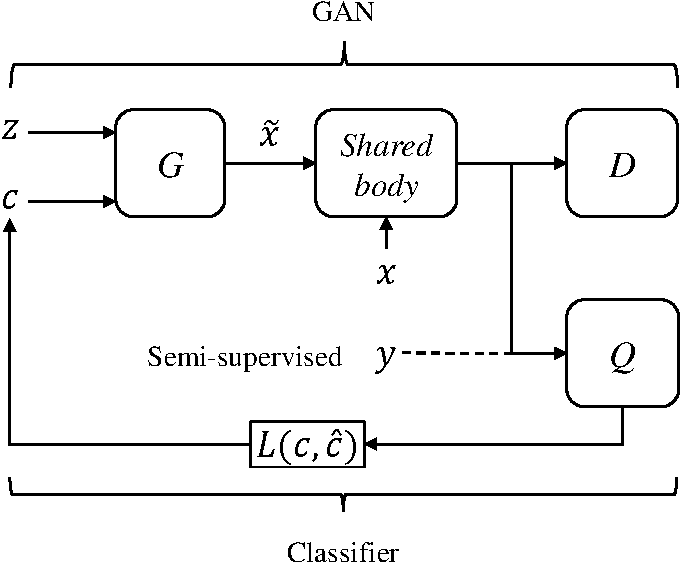
\includegraphics[scale=0.7]{Img/arch-cinfogan.pdf} 
  \bicaption[C-InfoGAN模型结构示意]
  {C-InfoGAN模型结构。无监督情况下,生成数据$\tilde{\bd{x}}$和真实数据$\bd{x}$参与训练,通过和$D$共享部分结构,$Q$网络可以将GAN模型学习到的特征加以利用,实现分类任务;在半监督情况下,一部分真实标签$y$会直接被$Q$网络利用,以得到更好的效果。优化$Q$网络的输出$\hat{c}$和隐变量$c$构成的损失函数$L(c,\hat{c})$来增加$Q$的分类准确率。}
  {The architecture of C-InfoGAN. In unsupervised case, the generated data $\tilde{\bd{x}}$ and the real data $\bd{x}$ are used for training. By sharing the body with $D$, $Q$ is able to using features learned by GAN framework to perform classification. In semi-supervised case, labels $y$ is directly fed into $Q$ to get better performance. We optimize the some loss function $L(c, \hat{c})$ of latent code $c$ and the output $\hat{c}$ of $Q$ to improve its accuracy.}
  \label{fig:c-infogan}
\end{figure}

\subsection{半监督分类方法}
%无监督的InfoGAN虽然已经取得非常好的生成效果,但是分类准确率并不是很高。一个自然的想法是通过添加少量标签信息能否使得生成效果更好,分类更准确?答案是肯定的。特别的,
当拥有少量标签信息时,C-InfoGAN可以利用这些标签进一步提升分类准确率和生成效果。同时将隐变量$c$直接绑定到真实的标签,实现精准调控。
%我们可以通过添加少量的标签信息,
%指导隐变量$c$更好地绑定到类别特征,实现精确地调控。
%另外,精确绑定到类别特征的隐变量$c$可以作为直接作为数据的真实标签使用。也就是说,当我们设定$c=1$的时候,生成器就会生成真实类别为`1'的数据。此时,$\argmax_c Q(c|\bd{x})$即可作为分类器的预测值。
不同于\citet{spurr2017guiding}将隐变量进一步划分为无监督版本$c_{us}$和半监督版本$c_{ss}$,同时设计两个辅助网络$Q_{us}$和$Q_{ss}$分别处理对应版本的隐变量;本文直接将标签信息加入$Q$网络,先用真实数据和标签训练,接着用生成数据和虚假标签(即隐变量$c$)来训练,这样做的目的是为了使真实标签的信息流入隐变量$c$中,或者可以说是用真实标签指导$c$绑定到正确的类别特征。使用和\ref{sec:ss-catgan}节中类似的方法,我们给出半监督C-InfoGAN的目标函数:
\begin{equation}
  \begin{split}
  \min_{G,Q}\max_D~ &V_{\text{ss-CIG}}(G,D,Q,\lambda_1,\lambda_2,\lambda_3) = 
  V_{\text{CIG}}(G,D,Q,\lambda_1,\lambda_2) + \\
  &\lambda_3 \E_{(\bd{x}^L, \bd{y}^L) \sim \mathcal{X}^L}
  \left[ \CE[\bd{y}^L, Q(y|\bd{x}^L)] \right].
  \end{split}
\end{equation}
模型结构参见图~\ref{fig:c-infogan}。


\section{InfoCatGAN}\label{sec:icg}
\subsection{无监督分类方法}\label{sec:icg-us}
在训练概率分类模型的过程中,通过优化条件熵可以将分类边界调整到更自然的位置(数据分散区域)\cite{grandvalet2005semi},因此CatGAN使用条件熵作为判别器判断真假数据的依据。但是,使用熵作为目标函数的一个缺点是没有类别指向性($K$个类别中任意一个都可以使$p(y|\mathbf{x})$呈单峰分布)。对于一个分类器,我们希望对于给定输入$\mathbf{x}$,有且仅有一个$k \in [K]$,使得$p(y=k|\mathbf{x})$最大,而对于任意$k' \neq k, ~p(y=k'|\mathbf{x})$均很小。然而问题在于训练数据集没有标注,每个数据样本对应的标签无从获得。

对于上述问题本文从InfoGAN中获得启发,提出InfoCatGAN模型。InfoGAN将输入噪声划分为$\mathbf{z}$和$\mathbf{c}$,实际上是对隐空间的结构进行了人为划分。一部分提供模型的容量,使得模型具有足够的自由度去学习数据的细节(高度耦合的特征);一部分提供隐变量,用于在学习过程中绑定到数据的显著特征(如:MNIST中的数字类别、笔画粗细、角度)。模型的核心思想如下:通过在隐空间构造一维隐变量$c$,在训练过程中将生成数据的类别标签与之绑定,使得可以通过$c$来控制生成数据的类别。
CatGAN对GAN的扩展主要在于改变了判别器的输出结构:为所有真实数据分配一个类别标签而对于虚假数据则保持一个不确定的状态。类似的,生成器应该致力于生成某个具体类别的数据而不是仅仅生成足够逼真的图片。

\begin{figure}[htbp]
  \centering
  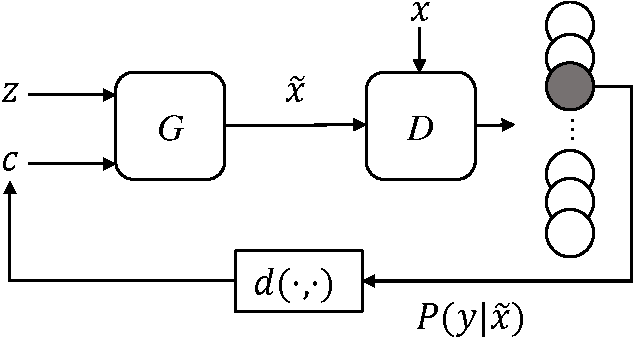
\includegraphics[width=.5\textwidth]{Img/icg-arch.pdf} 
  \caption{InfoCatGAN模型结构。图中$D$的输出为$P(y|\cdot)$。在训练生成器的时候,将判别器的输出$P(y|\tilde{\mathbf{x}})$和隐变量$c$通过某种度量$d(\cdot, \cdot)$建立联系使得条件概率的峰值与$c$的取值对应。}
  \label{fig:icg-arch}
\end{figure}

下面给出InfoCatGAN的损失函数:设$\mathbf{x} \in \mathcal{X}$为一个真实数据样本,$\tilde{\mathbf{x}} = G(\mathbf{z}, c)$为一个生成数据,其中$z\sim p_z$为噪声,$c\sim p_c$为隐变量。为了简单起见,这里只考虑$c$为一维离散随机变量,$p_c$为离散均匀分布。生成器$G = G(\mathbf{z}, c; ~\theta_G)$和判别器$D = D(\mathbf{x}; ~\theta_D)$均为可微深度神经网络,其中$\theta_G, ~\theta_D$分别为生成器和判别器的参数\footnote{为了简便起见,在无歧义的情况下通常省略网络参数。}。通过在$D$网络的最后一层做Softmax变换,可以直接将$D(x)$作为条件概率$p(y|x)$的估计。注意到式\eqref{eq:catgan-d}和\eqref{eq:catgan-g}可以重写为:
\begin{align}
  L_D^{\text{cat}} &= -I(X;Y)-
         \E_{\tilde{\mathbf{x}} \sim p_g}[H(p(y|\tilde{\mathbf{x}}))], \label{eq:lcatd} \\
  L_G^{\text{cat}} &= -I(\tilde{X}; Y), \label{eq:lcatg}
\end{align}
%%NOTE%%
% May have interaction with information bottleneck!
其中$X \sim p_{data}, ~\tilde{X} \sim p_g$分别表示真实数据和虚假数据对应的随机变量,$Y$表示未知标签对应的随机变量。从\eqref{eq:lcatd}、\eqref{eq:lcatg}式可以看出,CatGAN在优化数据与标签之间的互信息。互信息是常用的变量间相关性的衡量标准,所以本文用它作为生成器损失函数的正则项,由此得到InfoCatGAN的损失函数如下:
\begin{equation}
\label{eq:infocatgan}
\begin{split}
  L_D &= L_D^{\text{cat}}, \\ 
  L_G &= L_G^{\text{cat}} - \lambda_1 I(c; \tilde{\mathbf{x}}),
\end{split}
\end{equation}
其中$\lambda_1$为正则系数,可知当$\lambda_1 = 0$时,InfoCatGAN退化为CatGAN,模型结构见图~\ref{fig:icg-arch}。参考\eqref{eq:infogan-obj}式,$I(c; \tilde{\mathbf{x}})$可以放缩为$\E_{p(\mathbf{c},\tilde{\mathbf{x}})}[\log p(c|\tilde{\mathbf{x}})]$,在实现中通常使用交叉熵
\begin{equation}
  CE[\mathbf{c}, p(c|\tilde{\mathbf{x}})] = -\sum_{i=1}^K c_i \log p(c=c_i | \tilde{\mathbf{x}})
\end{equation}
来优化此项,这里的$\mathbf{c} \in \reals^K$是隐变量$c$经过one-hot编码之后的向量,$p(c|\tilde{\mathbf{x}})$可以用$D(\tilde{\mathbf{x}})$来近似。

\subsection{半监督分类方法}\label{sec:ss-infocatgan}
draft
作为CatGAN的扩展,InfoCatGAN能够很自然地适用于半监督的情况。假设$\mathcal{X}^L = \{\mathbf{x}_i^L\}_{i=1}^m$为$m$个有标签的样本,$\mathbf{y}_i^L \in \reals^K$为经过one-hot编码之后的标签向量。对于有标签的样本,$D(\mathbf{x}^L)$的分布信息可以明确获得,所以可以通过计算$y^L$和$p(y|\mathbf{x}^L)$之间的交叉熵:
\begin{equation}
  \label{eq:celoss}
  CE[\mathbf{y}^L, p(y|\mathbf{x}^L)] = -\sum_{i=1}^K y_i \log p(y=y_i | \mathbf{x}^L)
\end{equation}
来辅助判别器做出更精确的判断。半监督版本的InfoCatGAN损失函数如下:
\begin{equation}
  L_D^L = L_D + \lambda_2 \E_{(\mathbf{x}^L, \mathbf{y}^L) \sim \mathcal{X}^L}\left[ CE[\mathbf{y}^L, p(y|\mathbf{x}^L)] \right],
\end{equation}
其中$\lambda_2$为正则系数而生成器的损失函数同\eqref{eq:infocatgan}式:$L_G^L = L_G$.

\section{本章小结}
\textcolor{red}{To be written...}